\documentclass[a4paper,14pt]{extarticle}
\usepackage{../../tex-shared/report-layout}

\renewcommand{\mylabnumber}{4}
\renewcommand{\mylabtitle}{ЕЯ доступ к базе данных на основе алгоритма сопоставления с образцом}
\renewcommand{\mysubject}{Методы и средства искусственного интеллекта}
\renewcommand{\mylecturer}{Сметанина Т.И.}

\begin{document}
\begin{titlepage}
    
    \thispagestyle{empty}
    
    \begin{center}
        
        Министерство науки и Высшего образования Российской Федерации \\
        Севастопольский государственный университет \\
        Кафедра ИС
        
        \vfill

        Отчет \\
        по лабораторной работе №\mylabnumber \\
        \enquote{\mylabtitle} \\
        по дисциплине \\
        \enquote{\MakeTextUppercase{\mysubject}}

    \end{center}

    \vspace{1cm}

    \noindent\hspace{7.5cm} Выполнил студент группы ИС/б-17-2-о \\
    \null\hspace{7.5cm} Горбенко К. Н. \\
    \null\hspace{7.5cm} Проверил \\
    \null\hspace{7.5cm} \mylecturer

    \vfill

    \begin{center}
        Севастополь \\
        \the\year{}
    \end{center}

\end{titlepage}

\section{Цель работы}
Исследование алгоритма сопоставления с образцом и особенностей его применения
для формирования запросов к базам данных, а также для организации доступа к
базам данных на ограниченном подмножестве естественного языка.

\section{Постановка задачи}
Для базы данных, созданной в лабораторной работе 3, необходимо написать на языке
Лисп интерфейс, который позволяет выполнять ЕЯ-запросы с помощью алгоритма
сопоставления с образцом. Ответ на запрос должен также представляться на
естественном языке в виде списка слов предложения. Кроме запроса, заданного по
варианту задания, предусмотреть 5-6 различных дополнительных запросов.

\section{Ход работы}
Код программы:

\begin{lstlisting}
  (defun main ()
  (query '(Загрузить базу))
  
  (format t "Добавить маршрут из Москва в Краснодар с номером 418~%")
  (query '(Добавить маршрут из "Москва" в "Краснодар" с номером "418"))
  (format t "Добавить маршрут из Краснодар в Симферополь с номером 8~%~%")
  (query '(Добавить маршрут из "Краснодар" в "Симферополь" с номером "8"))
  
  (format t "Какие маршруты идут в город Симферополь~%")
  (selectQuery '(Какие маршруты идут в город "Симферополь"))
  
  (format t "Найти маршрут номер 8~%")
  (selectQuery '(Найти маршрут номер "8"))
  
  (format t "Какой маршрут идет в Краснодар~%")
  (selectQuery '(Какой маршрут идет в "Краснодар"))
  
  (format t "Показать все маршруты")
  (selectQuery '(Показать все маршруты))
  
  (format t "Изменить маршруты с конечной станцией Симферополь на Омск~%")
  (query '(Изменить маршруты с конечной станцией "Симферополь" на "Омск"))
  
  (format t "Изменить начальный маршрут у 1 номера на город Красноярск~%~%")
  (query '(Изменить начальный маршрут у "1" номера на город "Красноярск"))
  
  (format t "Показать все маршруты")
  (selectQuery '(Показать все маршруты))
  
  (format t "Выбрать маршруты с номерами от 1 до 9~%")
  (selectQuery '(Выбрать маршруты с номерами от "1" до "9"))
  )

(defvar *db* nil)

(defun insert (start end number)
  (push (list :start start :end end :number number) *db*)
  )

(defun savef (filename)
  (with-open-file (out filename :direction :output :if-exists :supersede)
    (with-standard-io-syntax
      (print *db* out)
      )
    )
  )

(defun loadf (filename)
  (with-open-file (in filename)
    (with-standard-io-syntax
      (setf *db* (read in))
      )
    )
  )

(defun select* ()
  (format t "~%")
  (format t "~%~{~{~a:~a~%~}~%~}" *db*)
  )

(defun where(&key start end number)
  #'(lambda (row)
      (and 
       (if start (equal (getf row :start) start) t)
       (if end (equal (getf row :end) end) t)
       (if number (equal (getf row :number) number) t)
       )
      )
  )

(defun update (where-func &key start end number)
  (setf *db*
        (mapcar
         #'(lambda (row)
             (when (funcall where-func row)
               (if start (setf (getf row :start) start))
               (if end (setf (getf row :end) end))
               (if number (setf (getf row :number) number))
               )
             row
             )
         *db*
         )
        )
  )

(defun selectByRangeNumber (startNumber endNumber)
  (remove-if-not #'(lambda (row) (and (> (parse-integer (getf row :number)) (parse-integer startNumber)) (< (parse-integer (getf row :number)) (parse-integer endNumber)))) *db*)
  )

(defun match (p d)
  (cond
    ;; правило 1
    ((and (null p) (null d)) t)
    
    ;; правило 2
    ((and (null d)
          (eq (car p) '$)
          (null (cdr p))) t)
    
    ;; один из списков исчерпан
    ((or (null p) (null d)) nil)
    
    ;; правило 3 и правило 4
    ((or (equal (car p) '?)
         (equal (car p) (car d)))
     (match (cdr p) (cdr d)))
    
    ;; правило 5 и 6
    ((eq (car p) '$)
     (cond ((match (cdr p) d) t)
       ((match p (cdr d)) t)))
    
    ;; правило 7 - сопоставление списков, включающих подсписки
    ((and (not (atom (car p)))
          (not (atom (car d)))
          (match (car p) (car d)))
     (match (cdr p) (cdr d)) )
    
    ;; правило 8 – подстановка значения в переменную
    ((and (atom (car p))
          (eq (car-letter (car p)) #\?)
          (match (cdr p)(cdr d)))
     (set (cdr-name (car p)) (car d)) t)
    
    ;; правило 9 - подстановка сегмента значений в переменную
    ((and (atom (car p))
          (eq (car-letter (car p)) #\$))
     (cond ((match (cdr p)(cdr d))
            (set (cdr-name (car p)) (list (car d)))
            t)
       ((match p (cdr d))
        (set (cdr-name (car p))
             (cons (car d)(eval (cdr-name (car p)))))
        t)))
    
    ;; правило 10 - обработка пакета ограничений, если в пакете есть «?»
    ((and (not(atom (car p)))
          (eq (caar p) 'restrict)
          (eq (cadar p) '?)
          (and-to-list
           (mapcar #'(lambda (pred)
                       (funcall pred (car d))) (cddar p))))
     (match (cdr p)(cdr d)))
    
    ;; правило 11 - обработка пакета ограничений, если в пакете есть «?V»
    ;; например: (match '((restrict ?V integerp evenp) b c) '(36 b c))
    ((and (not (atom (car p)))
          (not (atom d))
          (eq (caar p) 'restrict)
          (eq (car-letter (cadar p)) #\?)
          (and-to-list
           (mapcar #'(lambda (pred)
                       (funcall pred (car d))) (cddar p)))
          (match (cdr p)(cdr d)))
     (set (cdr-name (cadar p)) (car d))
     t)
    ))

(defun car-letter (x) (if (not (numberp x)) (car (coerce (string x) 'list))))

(defun cdr-name (x)
  (intern (coerce (cdr (coerce (string x) 'list)) 'string))
  )

(defun and-to-list (lis)
  (let ((res t))
    (dolist (temp lis res)
      (setq res (and res temp)))
    )
  )

(defun get-matches (p database)
  (remove-if-not #'(lambda (record) (match p record)) database)
  )

(defun query (q)
  (cond 
    ((match `($ загрузить $) q)
     (loadf "database.txt"))
    ((match `($ сохранить $) q)
     (savef "database.txt"))
    ((match `(Добавить $ из ?start в $ ?end $ с номером $ ?number) q)   
     (insert start end number))
    ((match `($ в город $ ?end) q)
     (setf temp (get-matches `($ :end ,end $) *db*))
     (if (null temp) "Маршрутов туда нет" temp))
    ((match `($ номер $ ?number) q)
     (setf temp (get-matches `($ :number ,number $) *db*))
     (if (null temp) "Маршрутов с таким номером нет" temp))
    ((match `($ идет в $ ?end) q)
     (setf temp (get-matches `($ :end ,end $) *db*))
     (if (null temp) "Отсутствуют маршруты с таким пунктом назначения" temp))
    ((match `($ все $) q)
     (select*))
    ((match `(Изменить $ конечной станцией ?end на ?endNew) q)
     (update (where :end end) :end endNew))
    ((match `(Изменить начальный маршрут у ?number номера на город ?start) q)
     (update (where :number number) :start start))
    ((match `(Выбрать $ с номерами от ?startNumber до ?endNumber) q)
     (selectByRangeNumber startNumber endNumber))
    )
  )

(defun selectQuery (q) 
  (setf temp (query q)) 
  (if (listp temp) 
      (format t "~%~{~{~a:~a~%~}~%~}" temp) 
      (format t "~%" temp)
      )
)
\end{lstlisting}

Результат работы программы: Содержимое файла до выполнения запросов – ((:START
"Москва" :END "Симферополь" :NUMBER "99") (:START "Евпатория" :END
"Санкт-Петербург" :NUMBER "2") (:START "Севастополь" :END "Москва" :NUMBER "1"))
\begin{figure}[H]
    \centering
    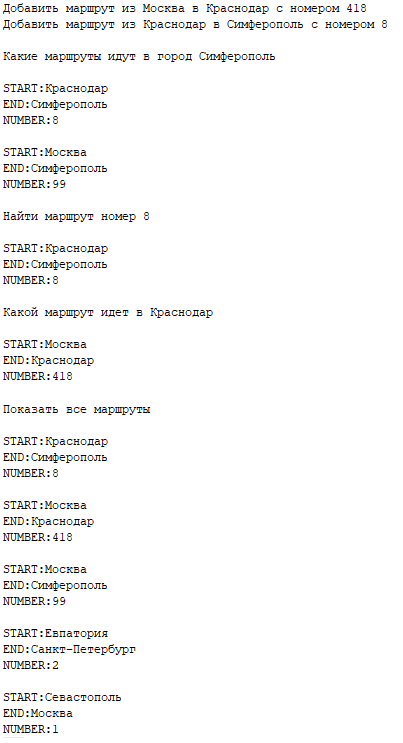
\includegraphics[width=.8\linewidth]{result1}
    \caption{Результат работы программы. Часть 1}
    \label{fig:result1}
\end{figure}

\begin{figure}[H]
  \centering
  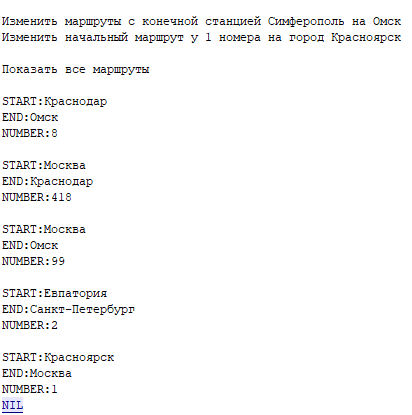
\includegraphics[width=.8\linewidth]{result2}
  \caption{Результат работы программы. Часть 2}
  \label{fig:result2}
\end{figure}

\begin{figure}[H]
  \centering
  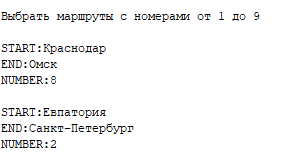
\includegraphics[width=.8\linewidth]{result3}
  \caption{Результат работы программы. Часть 3}
  \label{fig:result3}
\end{figure}

\section*{Выводы}
В ходе выполнения лабораторной работы был исследован алгоритм сопоставления с
образцом и особенности его применения для формирования запросов к базам данных,
а также для организации доступа к базам данных на ограниченном подмножестве
естественного языка.

\end{document}